\documentclass[UTF8]{ctexart}
\usepackage{geometry, CJKutf8}
\usepackage[affil-it]{authblk}
\usepackage[backend=bibtex,style=numeric]{biblatex}
\usepackage{hyperref}
\geometry{margin=1.5cm, vmargin={0pt,1cm}}
\setlength{\topmargin}{-1cm}
\setlength{\paperheight}{29.7cm}
\setlength{\textheight}{25.3cm}

% useful packages.
\usepackage{amsfonts}
\usepackage{amsmath}
\usepackage{amssymb}
\usepackage{amsthm}
\usepackage{enumerate}
\usepackage{graphicx}
\usepackage{multicol}
\usepackage{fancyhdr}
\usepackage{layout}
\usepackage{listings}
\usepackage{float, caption}

\lstset{
    basicstyle=\ttfamily, basewidth=0.5em
}

\begin{document}

\pagestyle{fancy}
\fancyhead{}
\lhead{梁育玮, 3230102923}
\chead{数据结构与算法第五次作业}
\rhead{\today}
\title{数据结构与算法第五次作业}

\author{梁育玮 3230102923
  \thanks{Electronic address: \texttt{liangyuwei631@gmail.com}}}
\affil{(Mathematics and Applied Mathematics 2302), Zhejiang University }


\date{\today}

\maketitle
\begin{abstract}
    本文档介绍了二叉搜索树中 \texttt{remove} 函数的实现和测试。首先,详细描述了 \texttt{detachMin} 和 \texttt{remove} 函数的实现思路,包括输入输出和具体步骤。接着,通过一系列测试验证了 \texttt{remove} 函数的正确性,展示了不同情况下节点删除后的树结构。
\end{abstract}

\section{\texttt{remove} 函数的实现}

以下是 \texttt{remove} 函数的实现思路。
\begin{itemize}
    \item \textbf{detachMin} 函数:
    \begin{itemize}
        \item 输入:当前节点指针 t,parent 节点指针 parent1
        \item 输出:最小节点指针
        \item 步骤:
        \begin{enumerate}
            \item 如果 t 为空,返回空指针
            \item 循环找到最小节点,更新 parent 节点指针
            \item 根据 parent 节点指针调整树结构
            \item 返回最小节点指针
        \end{enumerate}
    \end{itemize}
    \item \textbf{remove} 函数:
    \begin{itemize}
        \item 输入:要移除的元素 x,当前节点指针 t
        \item 步骤:
        \begin{enumerate}
            \item 循环查找要移除的节点,更新 parent 节点指针
            \item 如果未找到节点,返回
            \item 如果节点有一个或无子节点,使 parent 节点指向 t 的子节点 
            \item 如果节点有两个子节点,分离右子树的最小节点,并使 parent 节点指向最小节点
        \end{enumerate}
    \end{itemize}
\end{itemize}

因为我在实现的时候,将要求中的 “避免出现递归删除” 看成了 “避免出现递归”,所以我在实现的时候,没有使用递归,而只有循环,代价是代码的复杂度增加了,而且多了对 parent 节点的操作。但是能避免递归还是一件好事,编译器的编译速度或许能加快。

值得一提的是,代码思路来源于王何宇老师上课时画的一张很抽象的图 (见图\ref{fig:inspiration})\cite{DS_1029_course}。
\begin{figure}
    \centering
    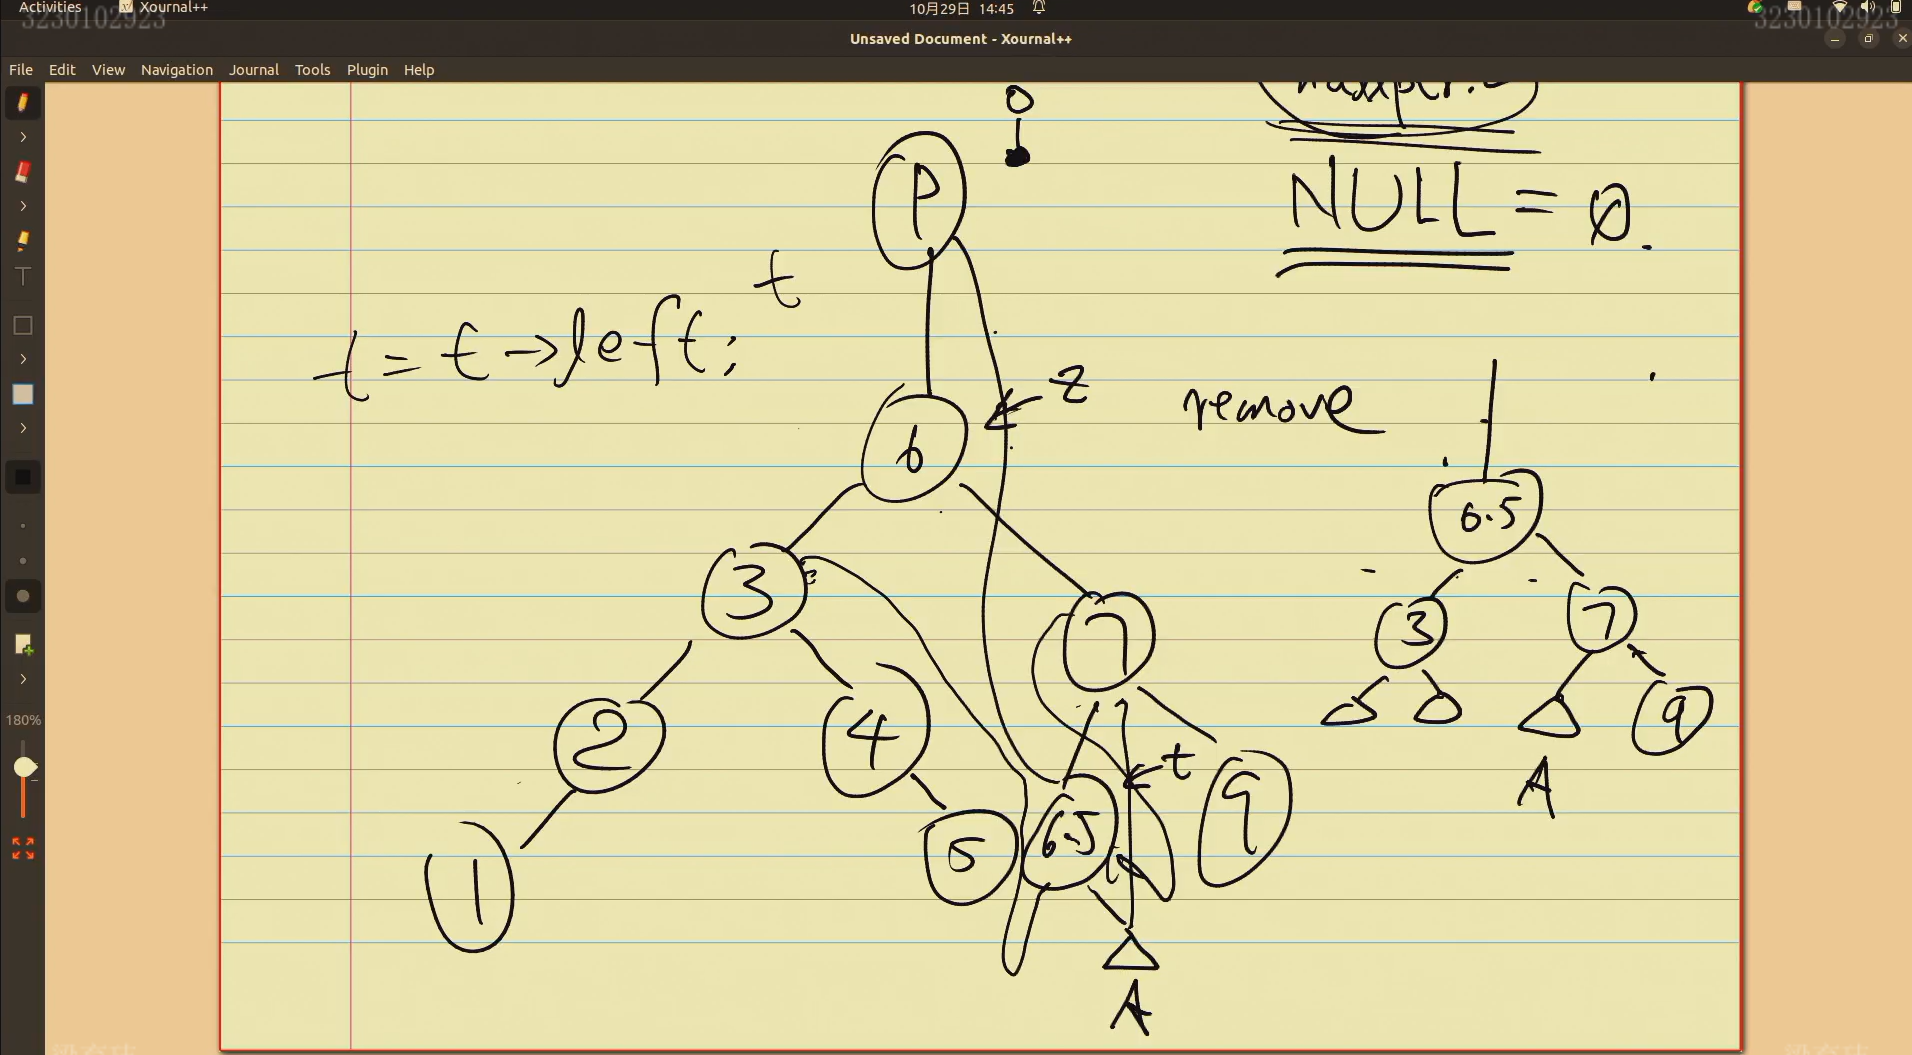
\includegraphics[width=0.7\textwidth]{./img/inspiration.png}
    \caption{代码思路来源(左边的树)。实现 7 指向 三角形, P 指向 6.5,6.5 指向 3 和 7 。}
    \label{fig:inspiration}
\end{figure}

\section{测试}

为了验证 \texttt{remove} 函数的正确性,我们编写了一个简单的测试程序。测试程序首先构建一个二叉搜索树,然后依次移除几个节点,并输出每次移除后的树结构。以下是测试程序的编译和运行结果:

\begin{verbatim}
Initial Tree:
3 5 7 10 12 15 18
Tree after removing 10:
3 5 7 12 15 18
Tree after removing 3:
5 7 12 15 18
Tree after removing 12:
5 7 15 18
Tree after removing 5:
7 15 18
Tree after removing 2:
7 15 18
\end{verbatim}

从测试结果可以看出,\texttt{remove} 函数能够正确地移除指定的节点,并保持二叉搜索树的性质。每次移除节点后,树结构都符合预期。

在测试过程中,删除 10 用于验证删除有两个子节点的情况,同时 10 也是根节点。删除 3 用于验证删除没有子节点的情况。删除 12 用于验证删除有两个子节点的情况,且右子树的最小节点是右子树的根节点。删除 5 用于验证删除只有一个子节点的情况,删除 2 用于验证节点找不到的情况,见图\ref{fig:remove}。
\begin{figure}[H]
    \centering
    \begin{minipage}[b]{0.45\textwidth}
        \centering
        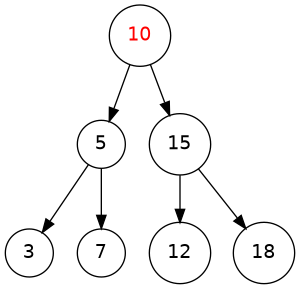
\includegraphics[height=5cm]{./img/1.png}
        \caption*{(a)删除 10 用于验证删除有两个子节点的情况}
    \end{minipage}
    \hfill
    \begin{minipage}[b]{0.45\textwidth}
        \centering
        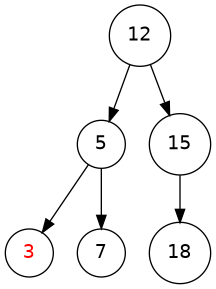
\includegraphics[height=5cm]{./img/2.png}
        \caption*{(b)删除 3 用于验证删除没有子节点的情况}
    \end{minipage}
    \vfill
    \begin{minipage}[b]{0.45\textwidth}
        \centering
        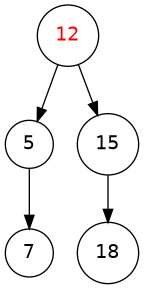
\includegraphics[height=5cm]{./img/3.png}
        \caption*{(c)删除 12 用于验证删除有两个子节点的情况,且右子树的最小节点是右子树的根节点}
    \end{minipage}
    \hfill
    \begin{minipage}[b]{0.45\textwidth}
        \centering
        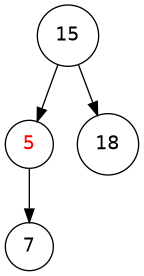
\includegraphics[height=5cm]{./img/4.png}
        \caption*{(d)删除 5 用于验证删除只有一个子节点的情况。}
    \end{minipage}
    \caption{树的删除操作展示}
    \label{fig:remove}
\end{figure}

valgrind 调试后没发现内存泄漏。

\begin{thebibliography}{9}

\bibitem{DS_1029_course}
Zhejiang University, 
\href{https://www.example.com}{\textit{数据结构和算法 2024-10-29第6-8节}, 
王何宇, 紫金港西1-215}, 
\url{https://classroom.zju.edu.cn/livingroom?course_id=64093&sub_id=1405399&tenant_code=112&ts=5010}.

\end{thebibliography}


\end{document}

%%% Local Variables: 
%%% mode: latex
%%% TeX-master: t
%%% End: 